\documentclass[aspectratio=169,10pt]{beamer}
\usetheme{Boadilla}
\usepackage{graphicx,booktabs}
\title{Light-flavour backgrounds and photon veto proposals}
\subtitle{v3 Stage 2; fixed 1,091-chunk BDT; full 1,200-chunk Zcc/Zss campaigns}
\author{FCC-ee $\Lambda_b\to\Lambda\gamma$ analysis}
\date{4 October 2026}
\begin{document}
\frame{\titlepage}

\begin{frame}{Question and frozen samples}
\begin{itemize}
\item Compare direct signal, nonmatched Zbb/Zcc/Zss, and forced $\Lambda\eta$/$\Lambda\pi^0$ candidates at fixed BDT score $\geq0.9538269639$.
\item Zbb: 1,091 v3 chunks, 395,623,929 processed input events. Zcc: 1,200 chunks, 499,786,495 events. Zss: 1,200 chunks, 499,842,440 events.
\item Direct Physics signal: 100,002 generated direct decays. Forced $\eta$ and $\pi^0$: 100,000 and 100,005 generated direct decays. Both charge conjugates included.
\item Plot physically weighted \emph{candidate rows}, with 5.4--5.9 GeV as provisional reconstructed peak. Truth labels are diagnostic after candidate construction.
\end{itemize}
\end{frame}

\begin{frame}{Normalization and paired proposal}
\begin{itemize}
\item $N_Z=6\times10^{12}$; $\mathcal B(Z\to b\bar b)=0.15$, $\mathcal B(Z\to c\bar c)=0.1203$, $\mathcal B(Z\to s\bar s)=0.156$ as a down-type flavour-equality scenario.
\item Each inclusive weight is $N_Z\mathcal B(Z\to q\bar q)/N_{\rm processed,q}$, applied to nonmatched candidate rows. Forced modes stay separate from inclusive Zbb.
\item Four paired stages: fixed BDT; add Armenteros box $0.67\leq|\alpha|\leq0.78$, $0.075\leq q_T\leq0.120$ GeV; add $\pi^0$ photon-pair veto $\pm20$ MeV; add $\eta$ veto $\pm50$ MeV.
\item All stages use reconstructed quantities only. Windows and score remain proposals pending PI review and angular response work.
\end{itemize}
\end{frame}

\begin{frame}{Expected reconstructed mass: all components, linear scale}
\centering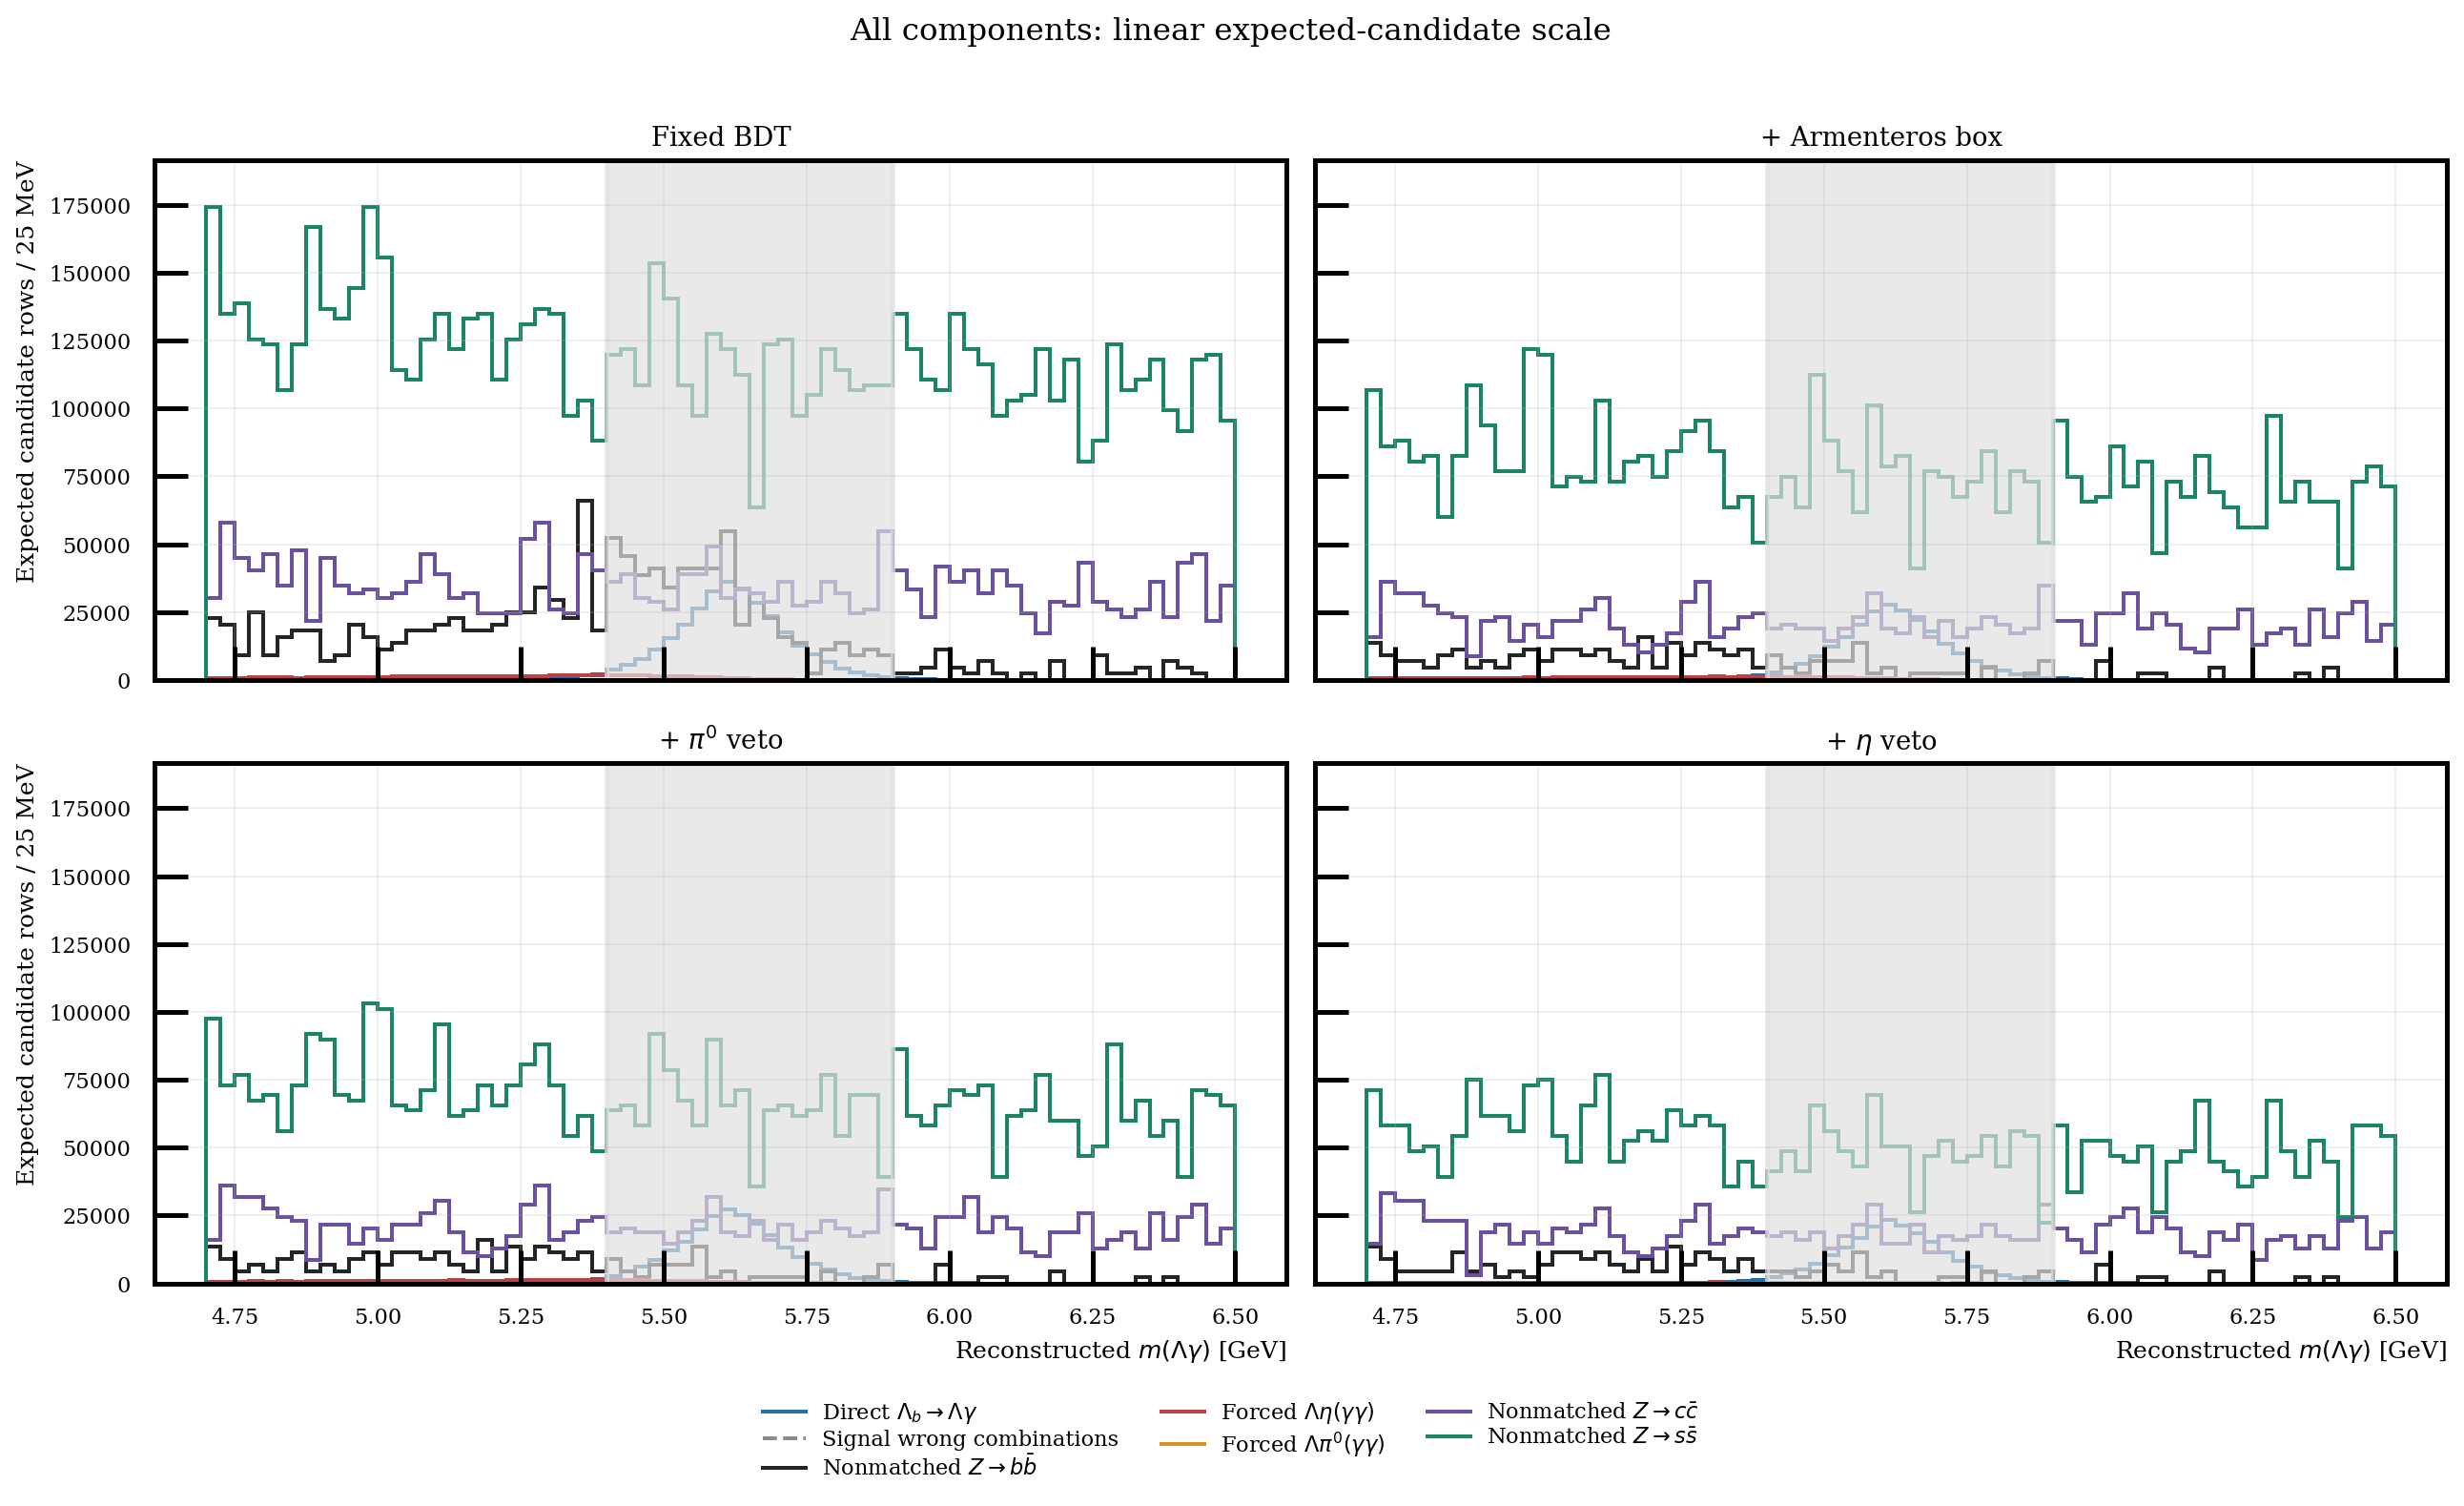
\includegraphics[height=.83\textheight]{figures/sequence_mass_linear.png}
\end{frame}

\begin{frame}{Expected reconstructed $\cos\theta_p$: all components, linear scale}
\centering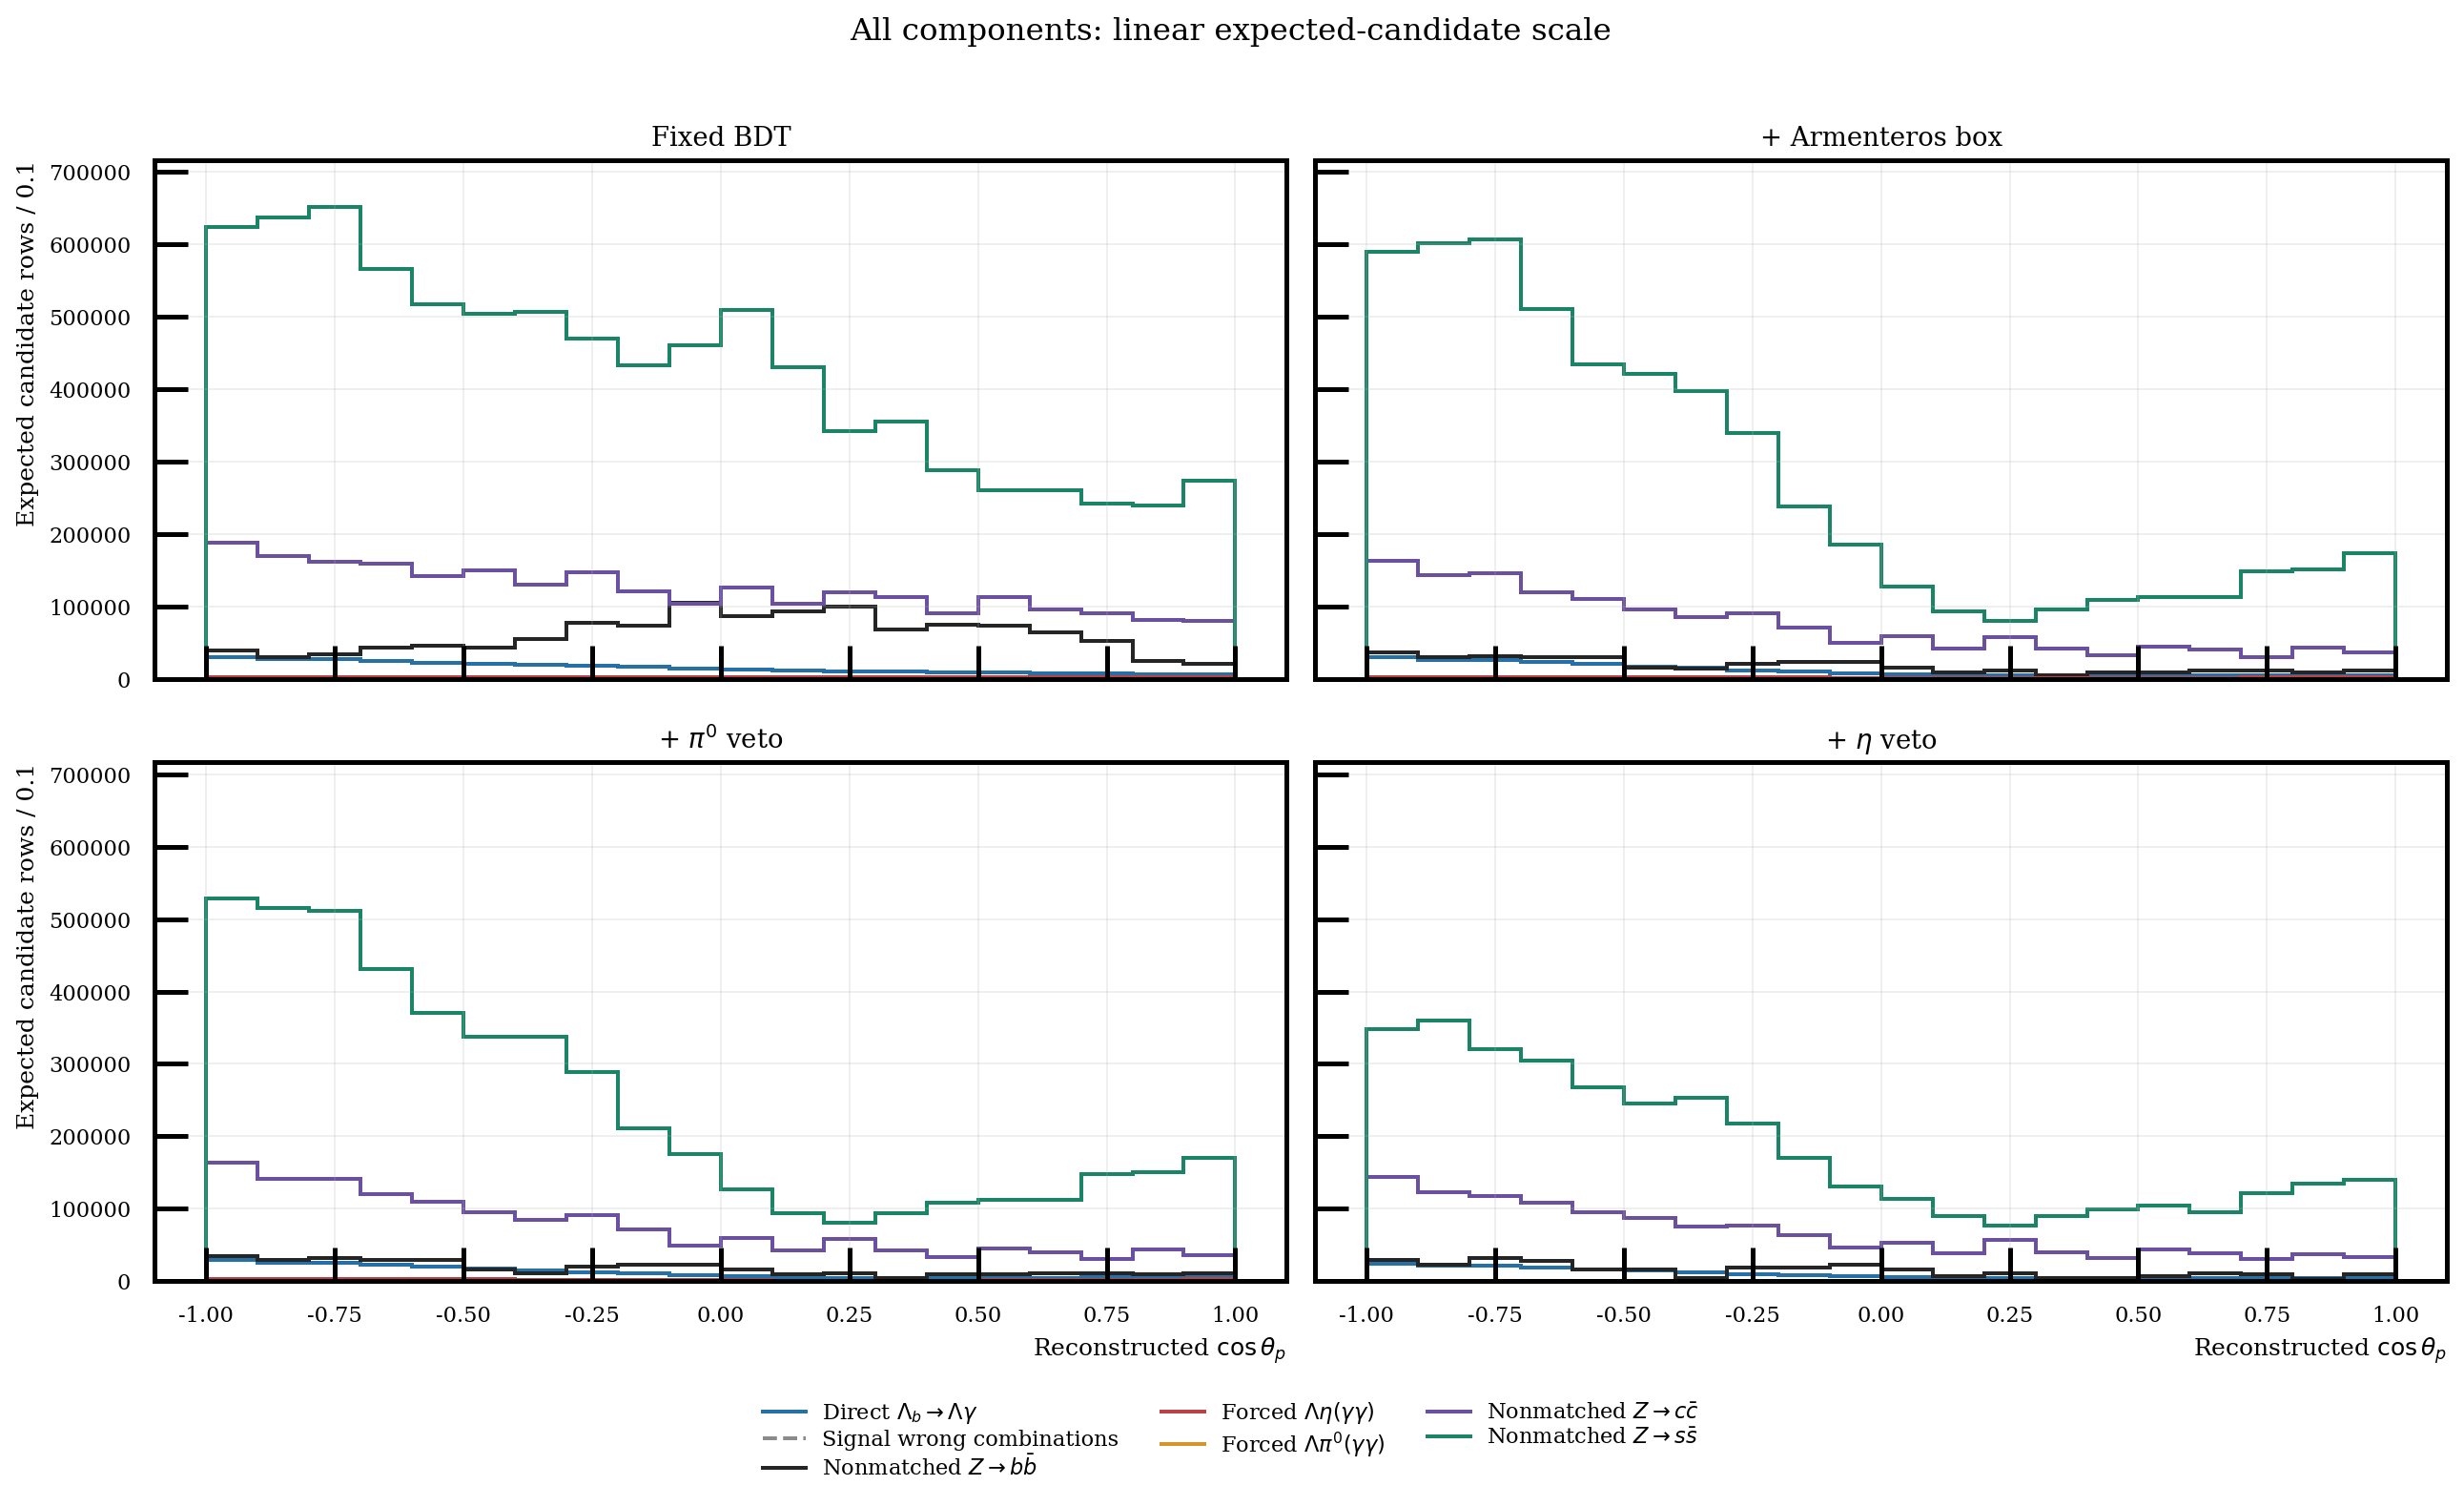
\includegraphics[height=.83\textheight]{figures/sequence_angle_linear.png}
\end{frame}

\begin{frame}{Peak expected candidates (5.4--5.9 GeV)}
\scriptsize
\begin{tabular}{lrrrrrr}
\toprule
Step & Signal & Zbb & Zcc & Zss & Forced $\eta$ & Forced $\pi^0$\\
\midrule
BDT & 301,335 & 550,523 & 677,338 & 2,286,433 & 13,136 & 107\\
+ Armenteros & 231,473 & 79,621 & 410,158 & 1,486,837 & 9,844 & 84\\
+ $\pi^0$ veto & 228,827 & 79,621 & 410,158 & 1,308,940 & 9,785 & 66\\
+ $\eta$ veto & 194,757 & 61,422 & 363,943 & 962,511 & 1,924 & 60\\
\bottomrule
\end{tabular}
\vspace{1.3em}

\small Zcc peak rows: 469 $\to$ 252; Zss: 1,221 $\to$ 514. Final candidate-count MC 95\% intervals: Zcc 320,391--411,762; Zss 881,089--1,049,433; Zbb 40,477--89,366. These omit normalization and detector systematics.
\end{frame}

\begin{frame}{Smaller components: mass, linear scale}
\centering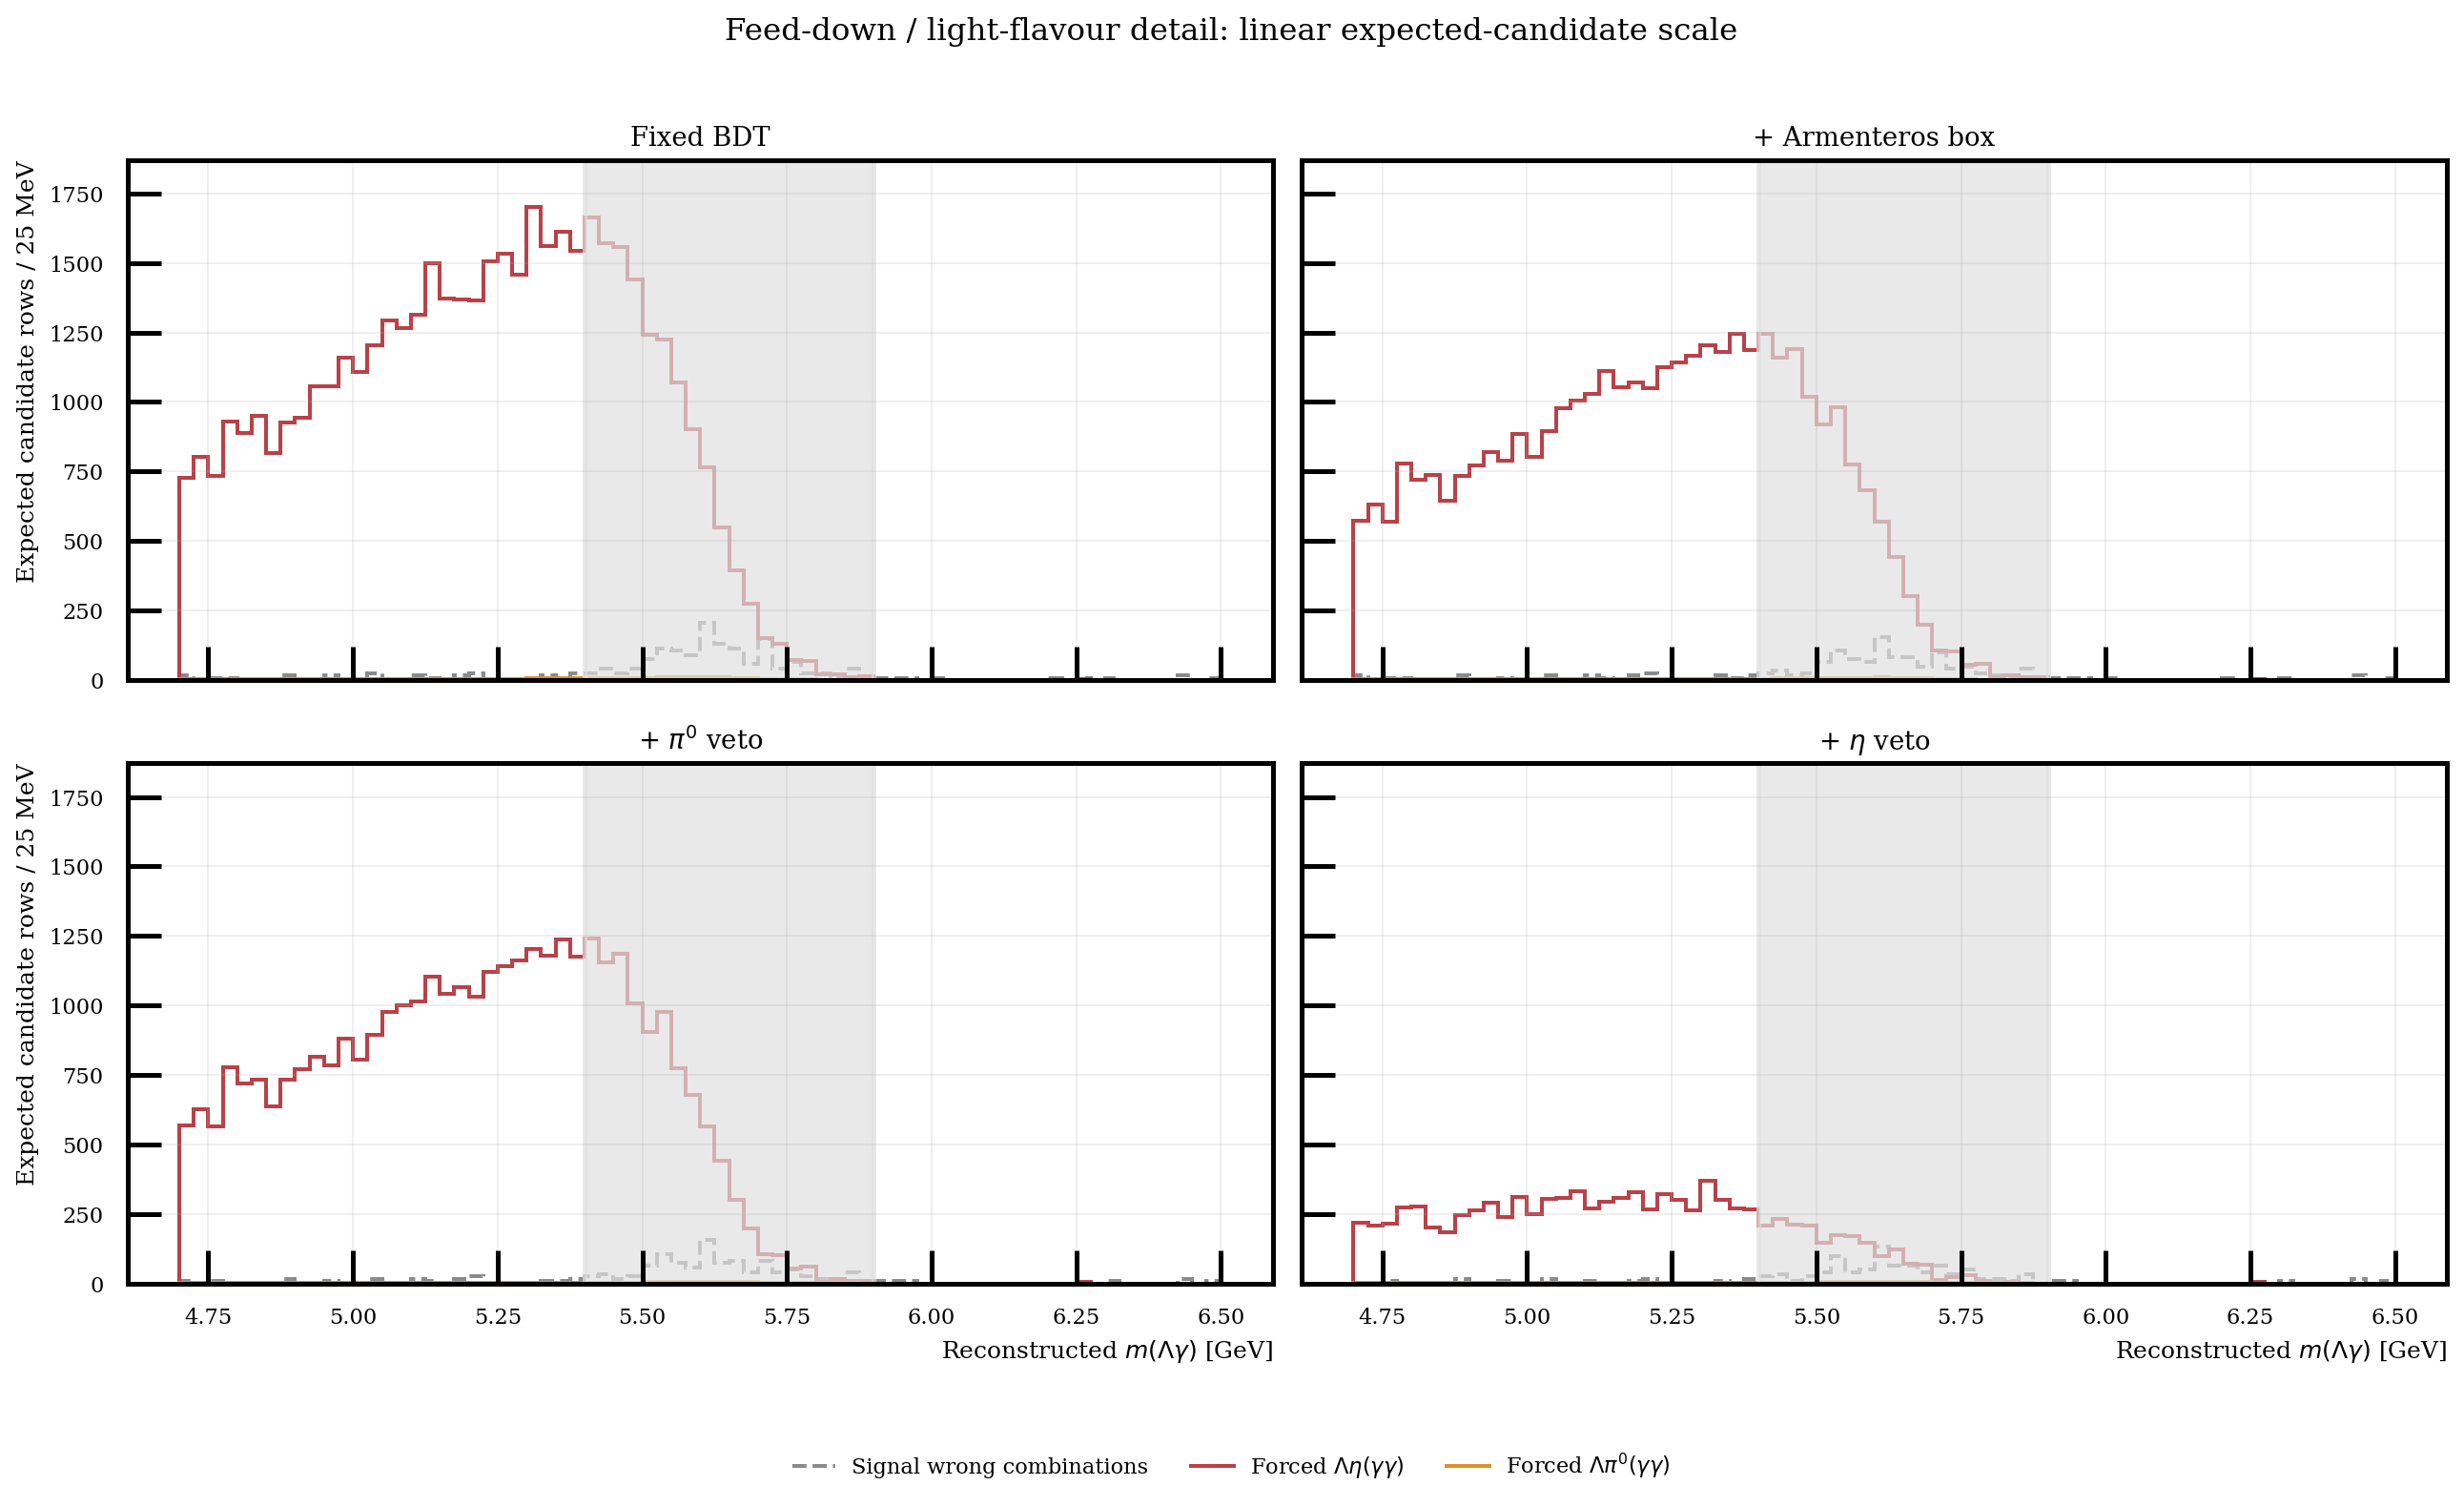
\includegraphics[height=.83\textheight]{figures/sequence_mass_detail_linear.png}
\end{frame}

\begin{frame}{Smaller components: $\cos\theta_p$, linear scale}
\centering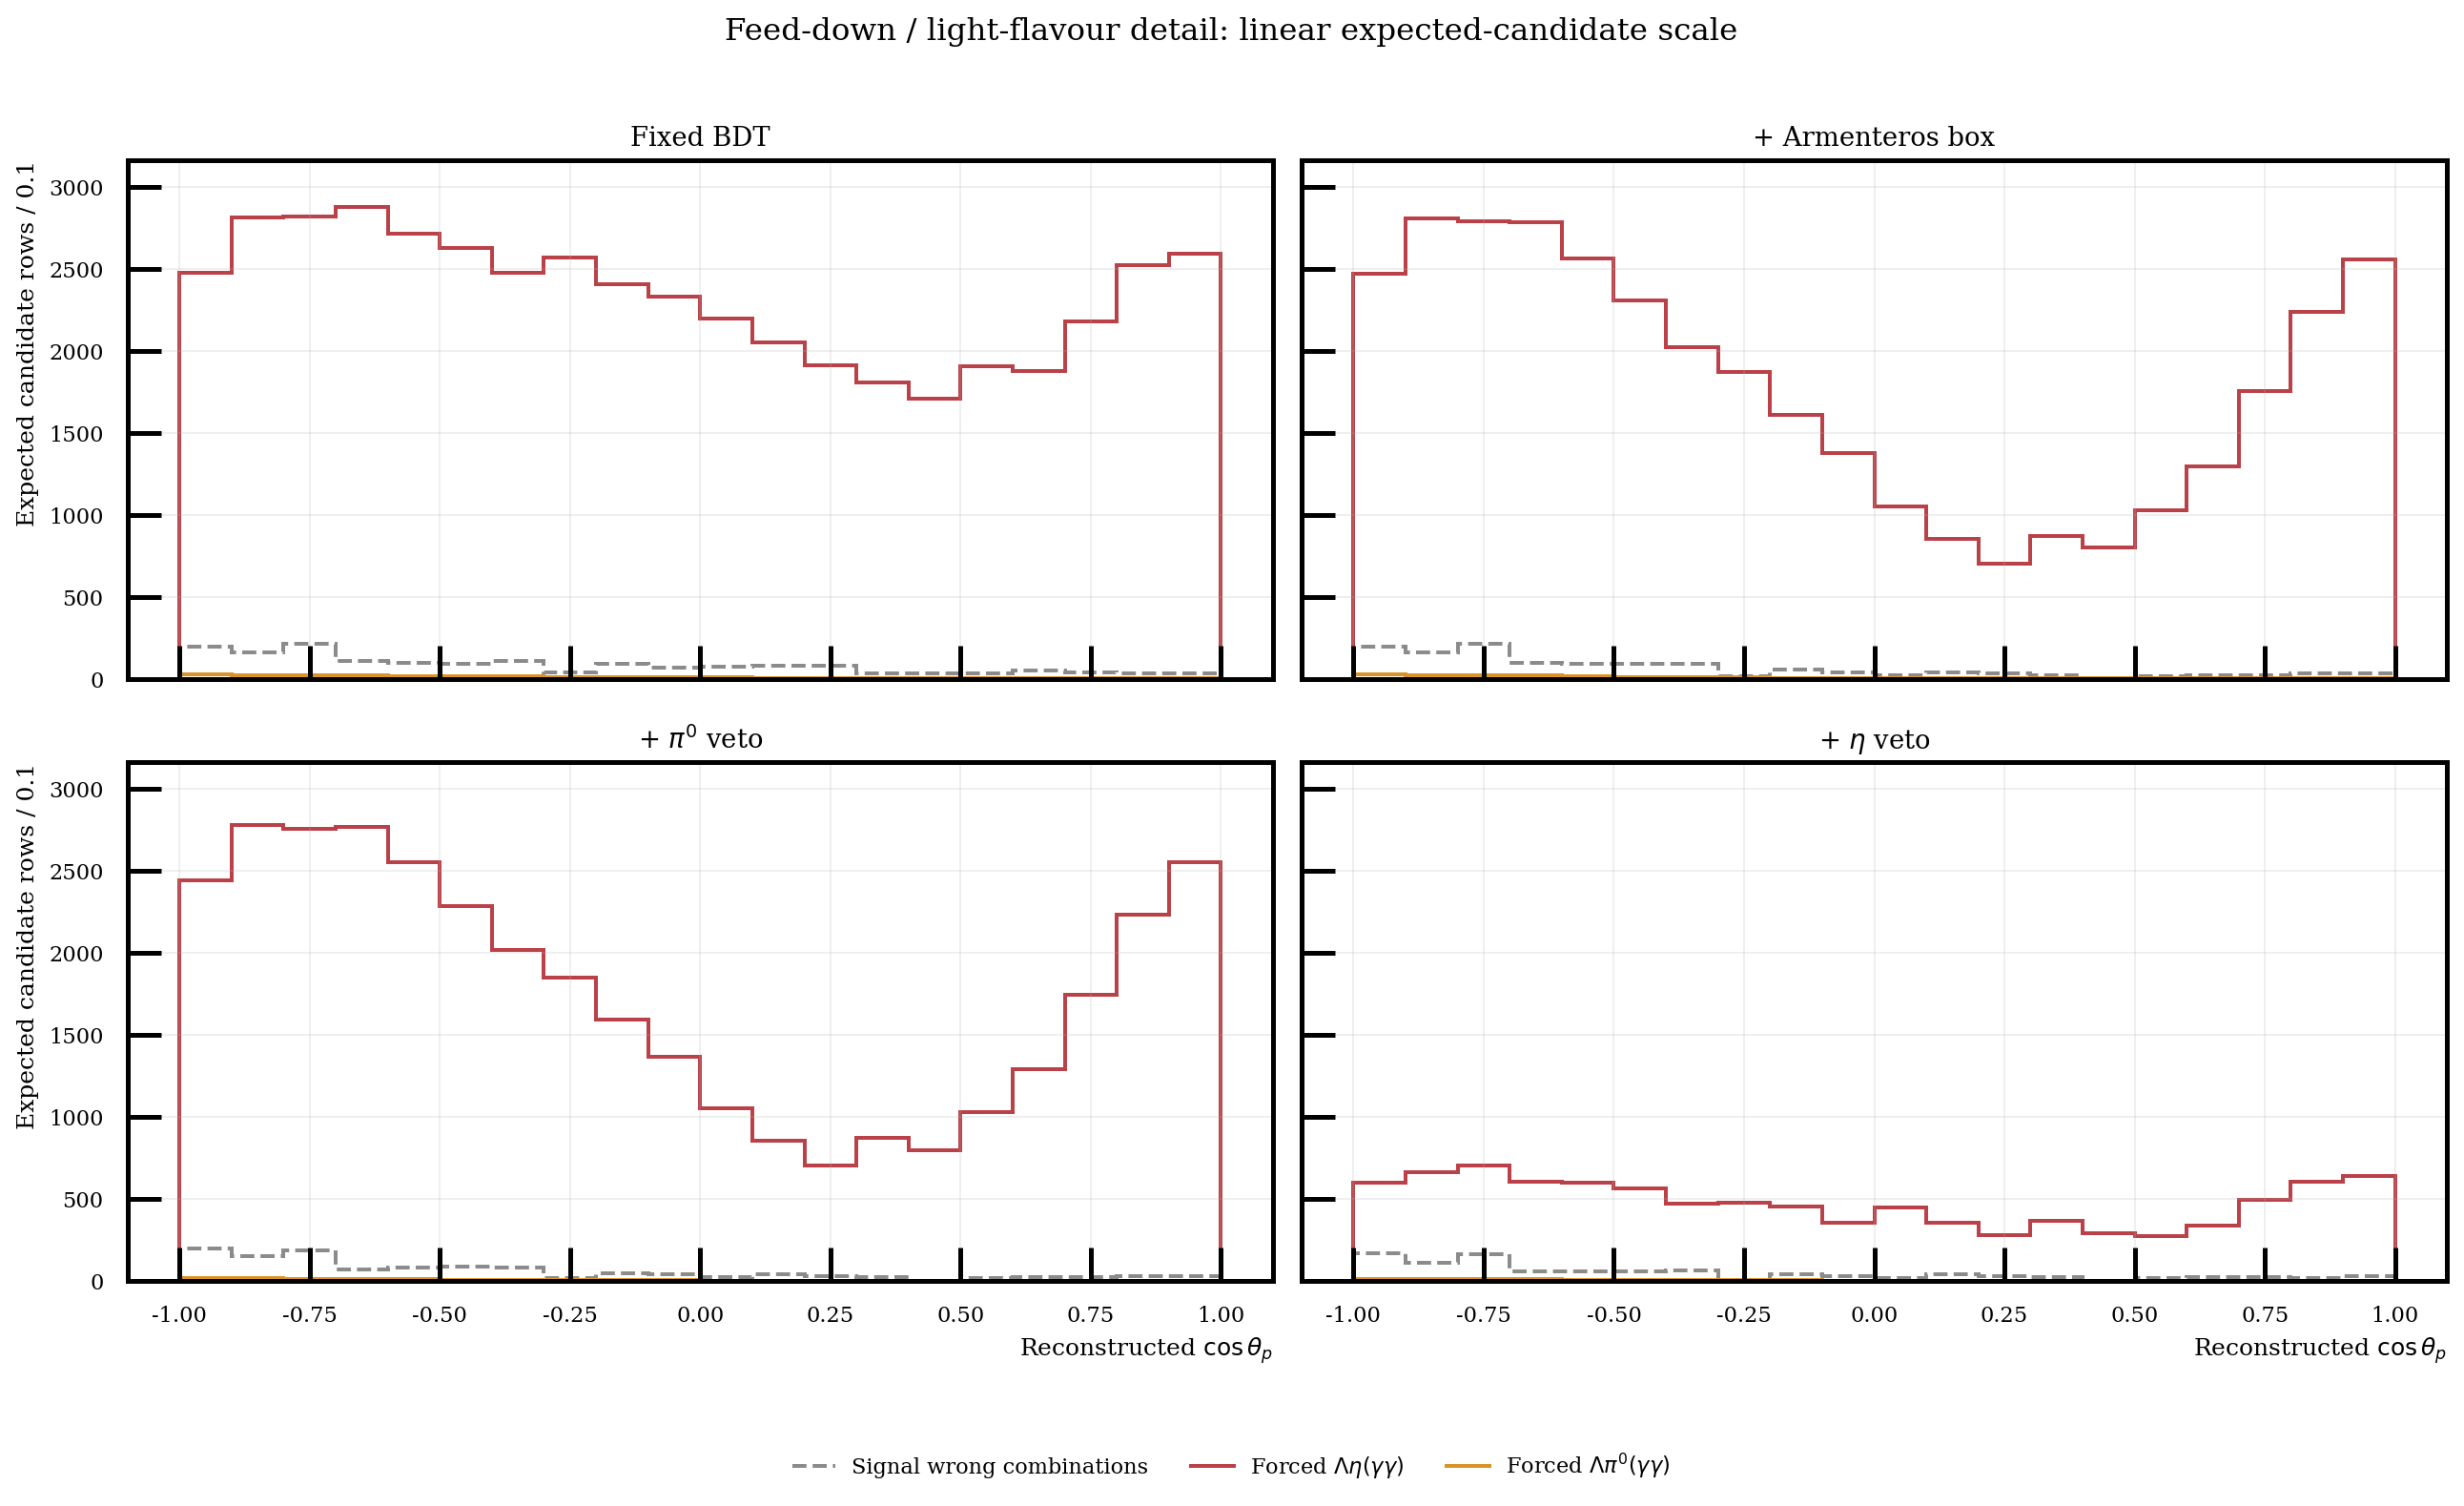
\includegraphics[height=.83\textheight]{figures/sequence_angle_detail_linear.png}
\end{frame}

\begin{frame}{Forced $\pi^0$ mass detail, linear scale}
\centering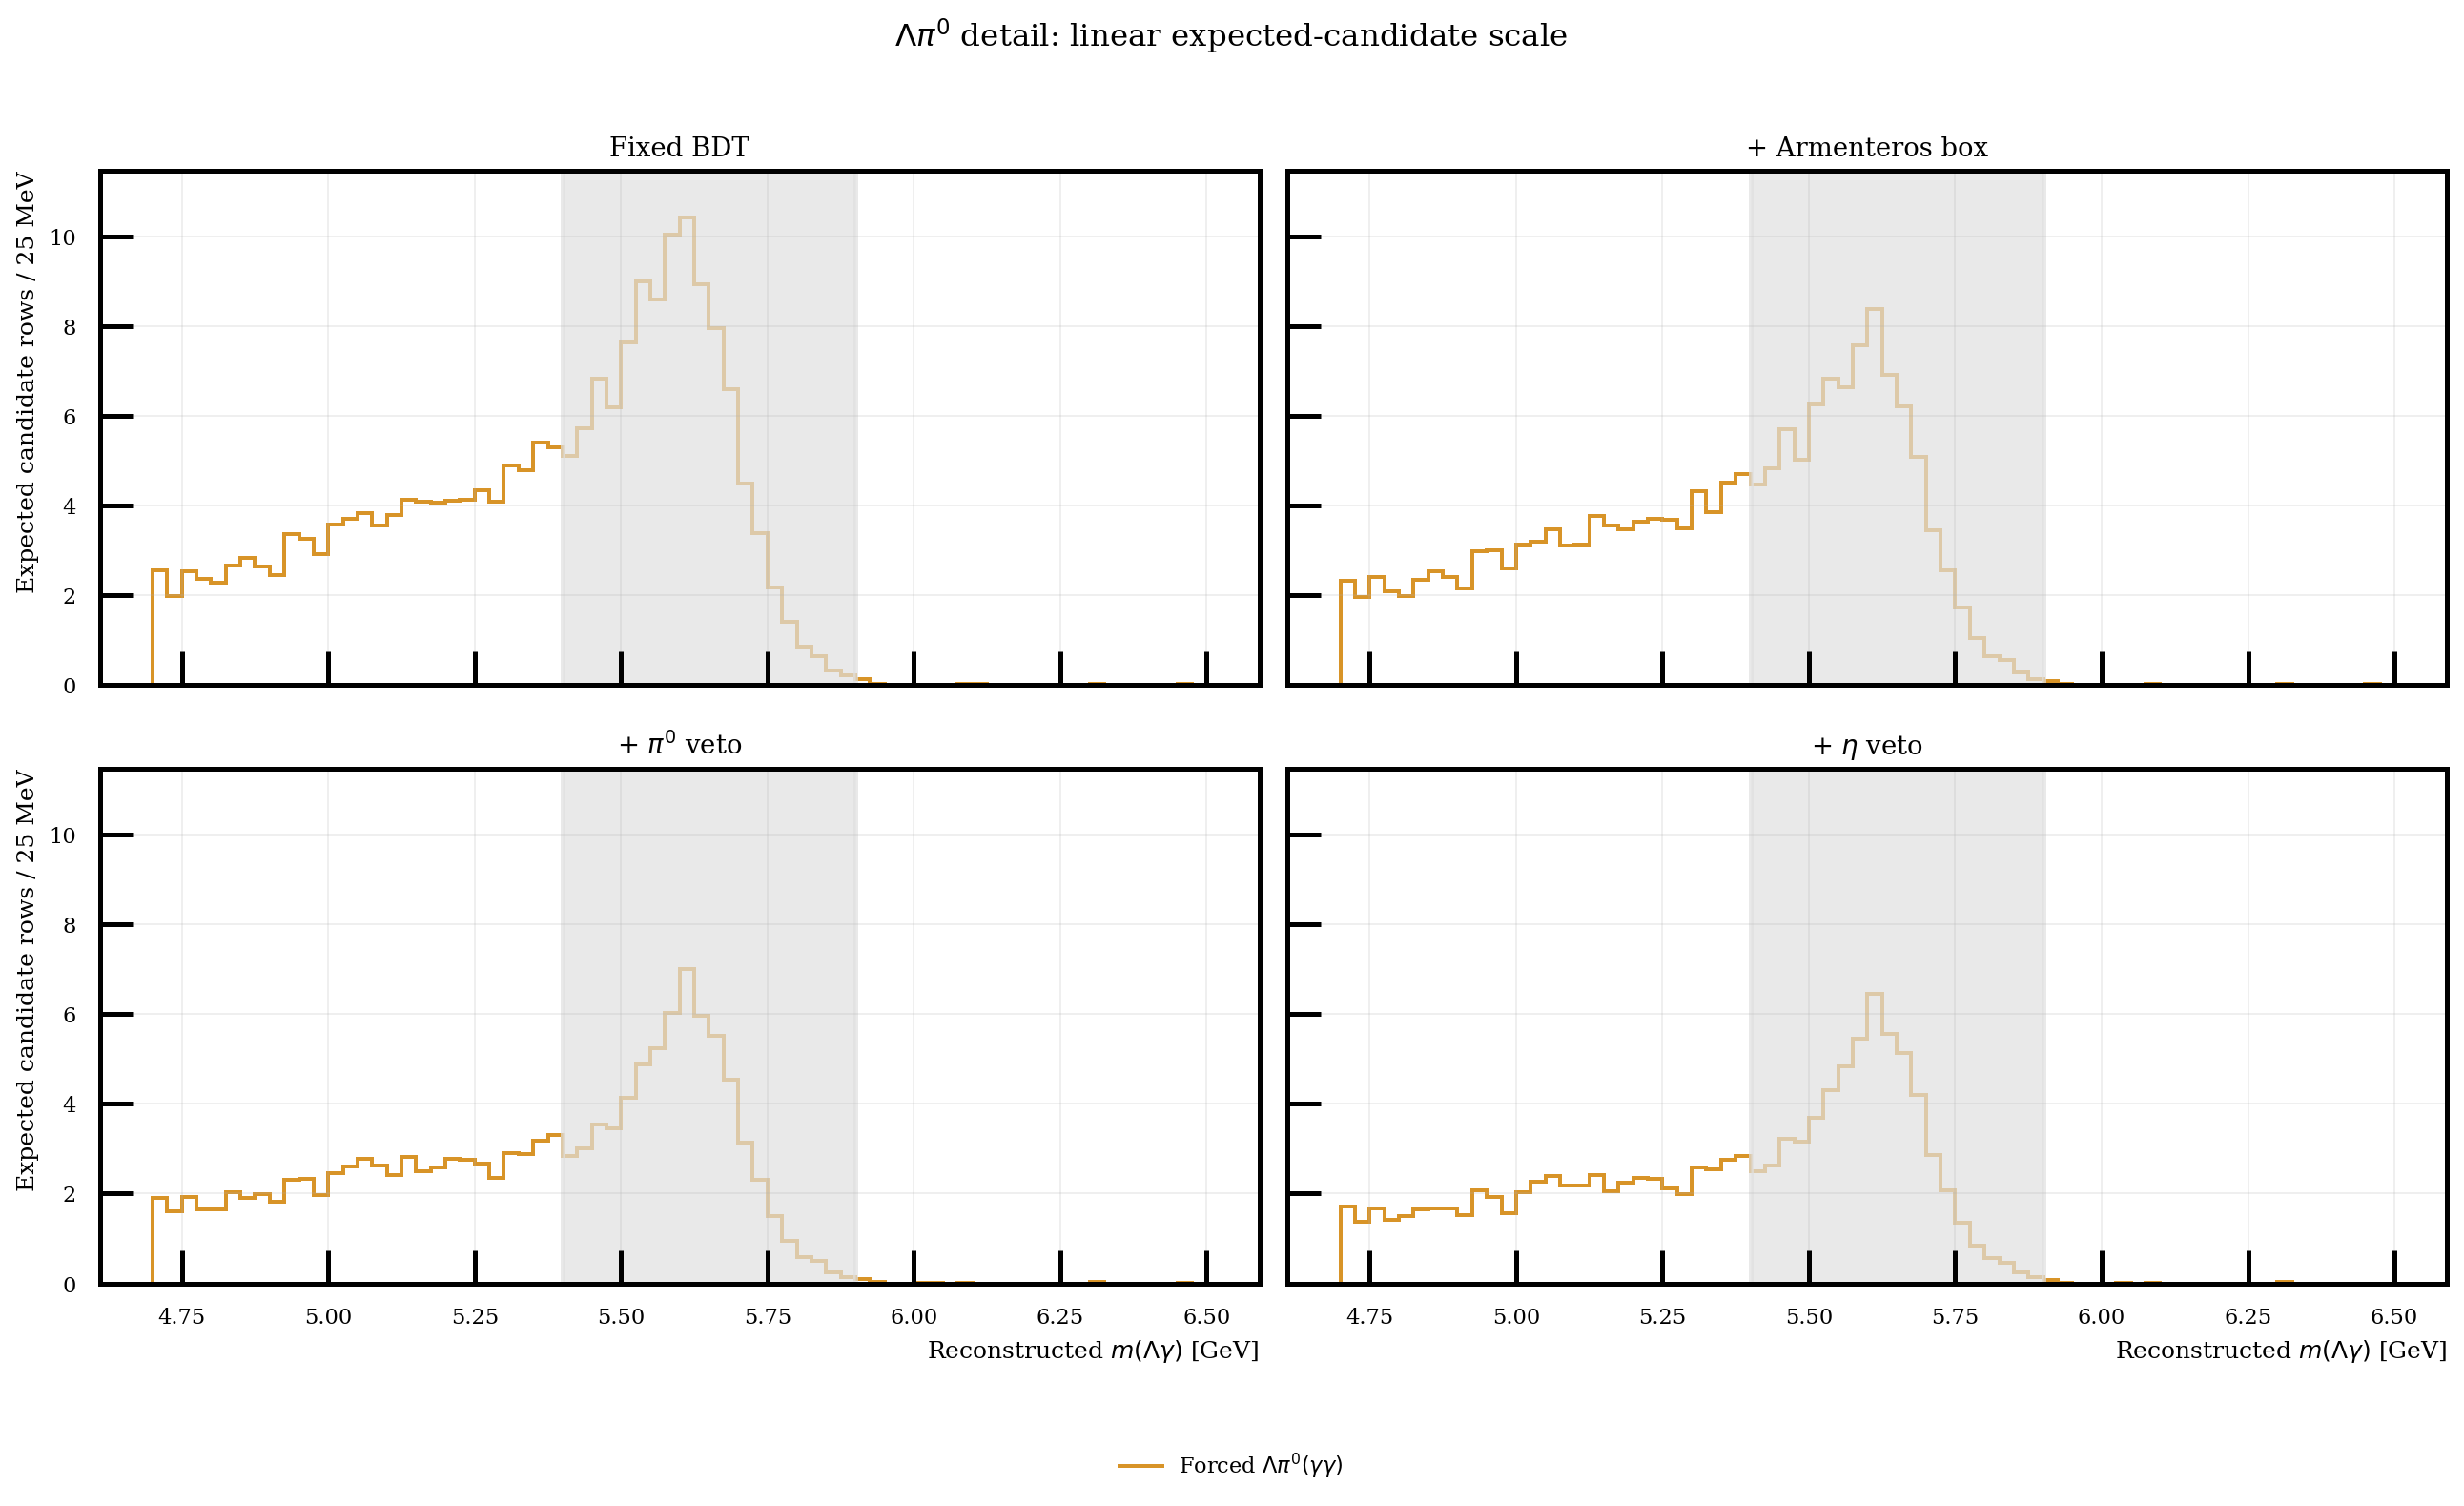
\includegraphics[height=.83\textheight]{figures/sequence_mass_pi0_linear.png}
\end{frame}

\begin{frame}{Zss truth: a real $\Lambda$ pair dominates}
\centering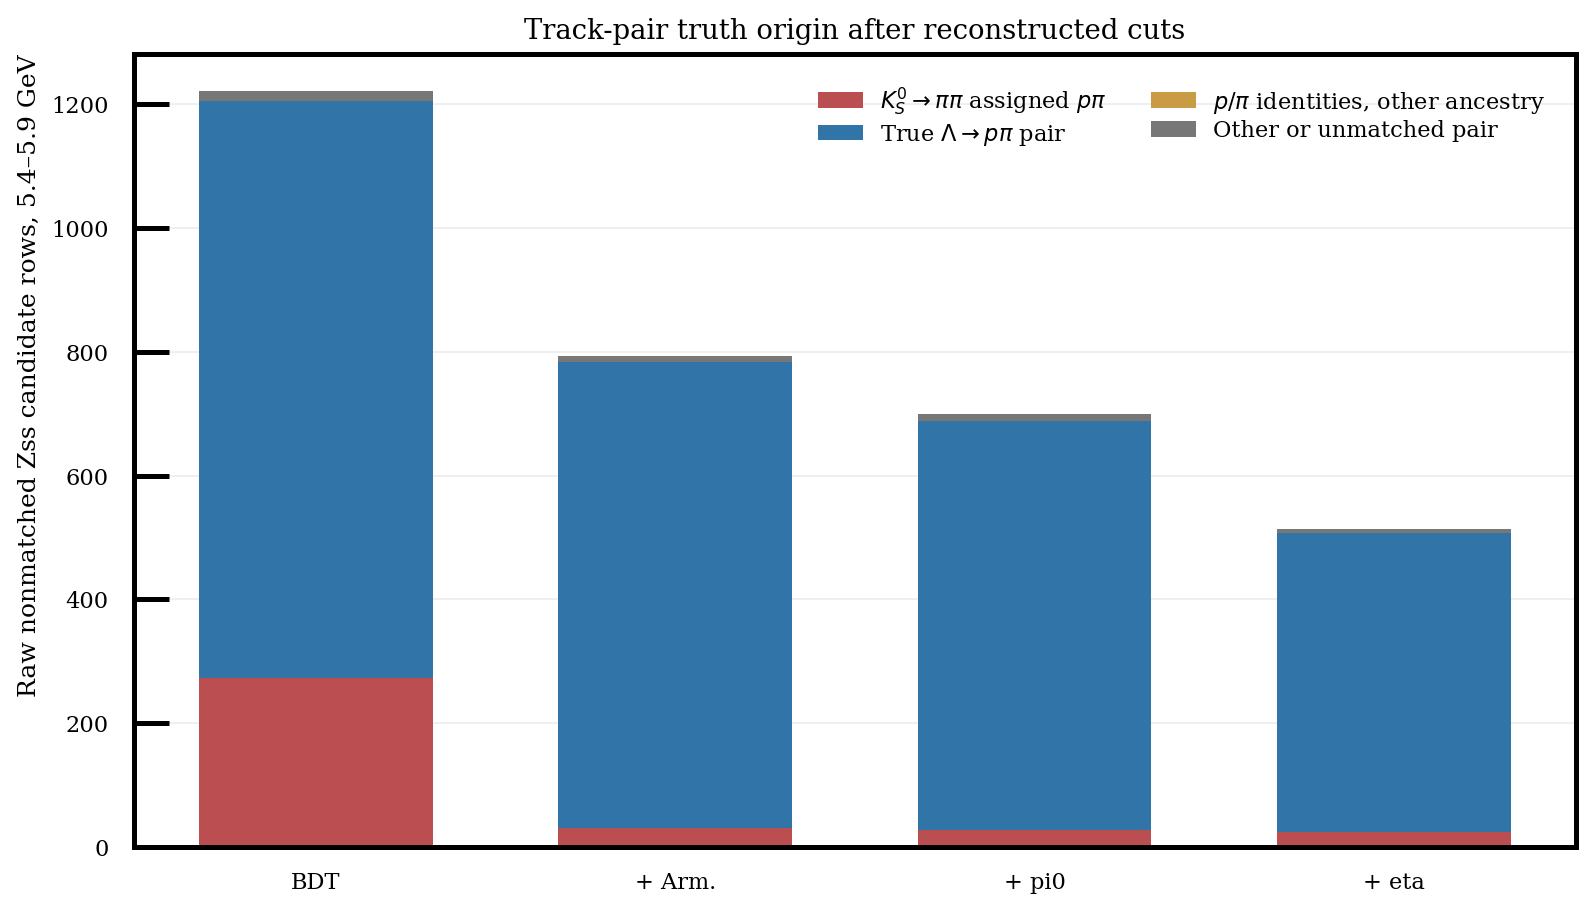
\includegraphics[height=.78\textheight]{figures/zss_peak_pair_origin.png}
\vspace{-.5em}

\scriptsize The Armenteros box removes 242/273 true $K^0_S$ pairs, but 752/932 true $\Lambda$ background pairs survive. Direct signal retention is 76.8\%.
\end{frame}

\begin{frame}{Photon origins in Zss}
\centering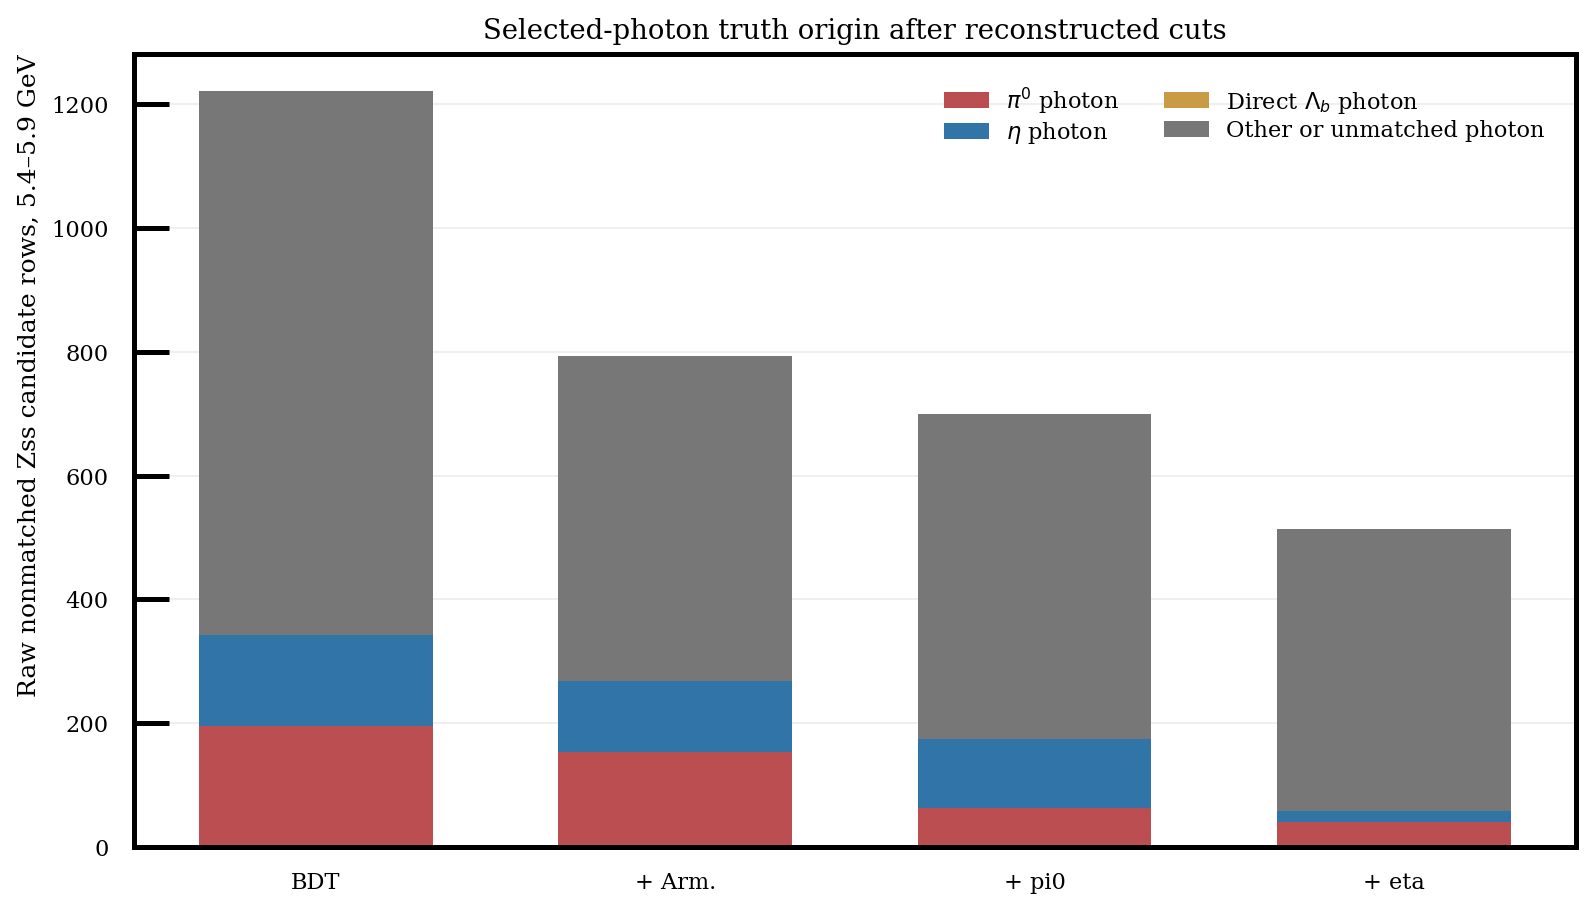
\includegraphics[height=.78\textheight]{figures/zss_peak_photon_origin.png}
\vspace{-.5em}

\scriptsize After all proposals, 429/514 peak candidates combine a true $\Lambda$ pair with a photon outside the $\pi^0/\eta$-parent categories. Parent-quark links need generator-record interpretation.
\end{frame}

\begin{frame}{Tracing the selected photon through the stored MC chain}
\centering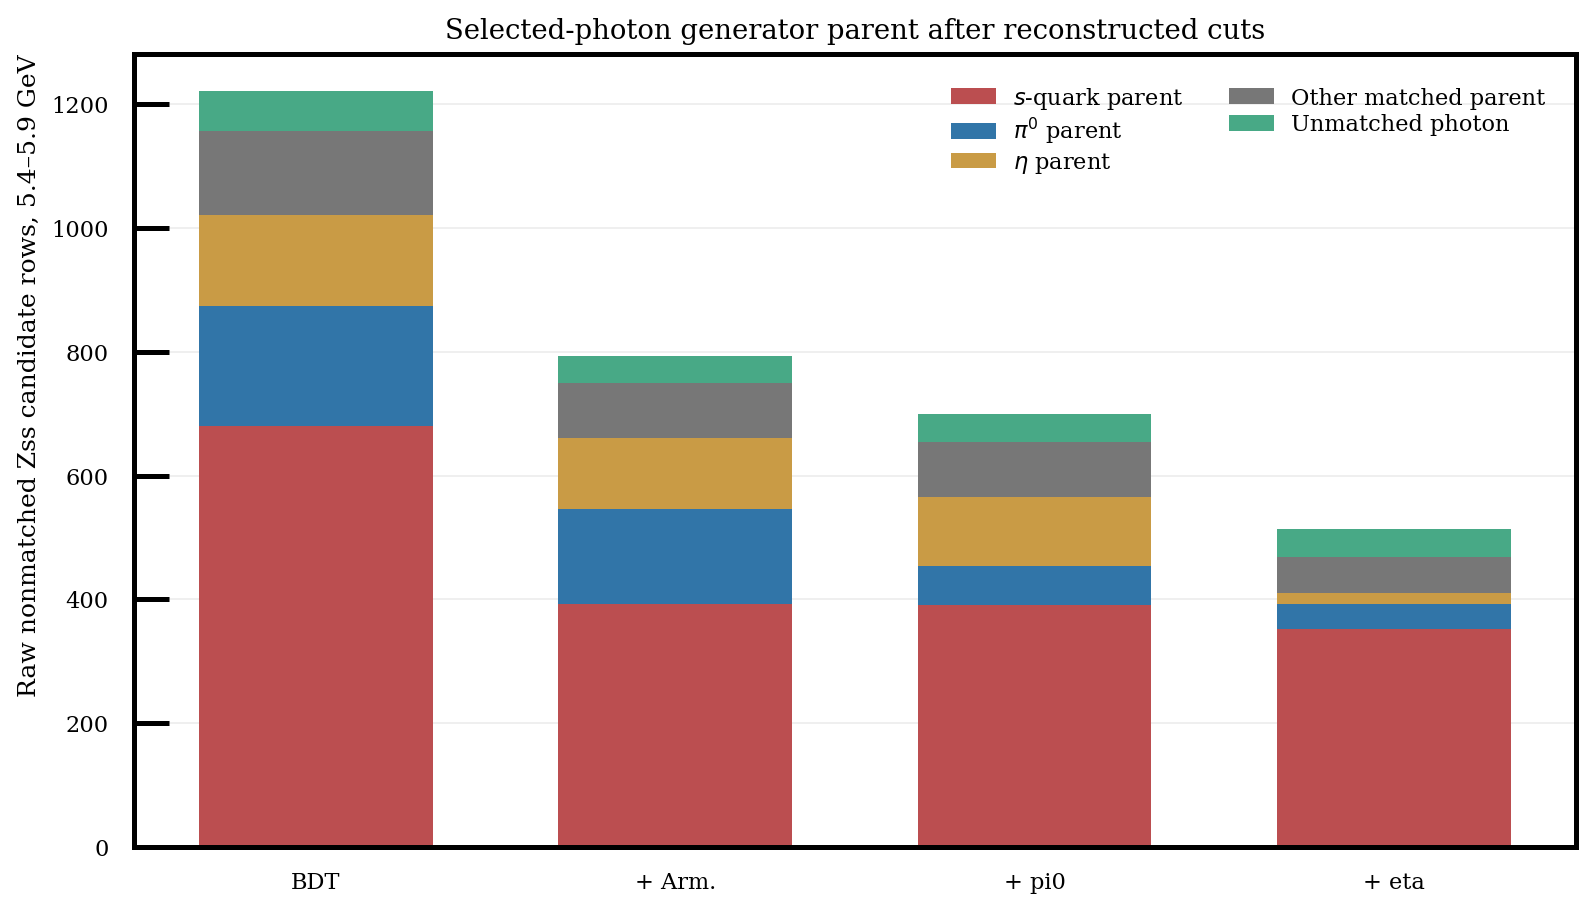
\includegraphics[height=.77\textheight]{figures/zss_peak_photon_source.png}
\vspace{-.5em}

\scriptsize Final peak: 352/514 photons have a recorded $s$-quark parent; 347 of those reach a Z within four stored ancestor generations. The first-parent chain supports a strange-parton origin, while the full event graph is needed to name the shower mechanism.
\end{frame}

\begin{frame}{Follow-up: reconstructed $\Lambda$ displacement}
\centering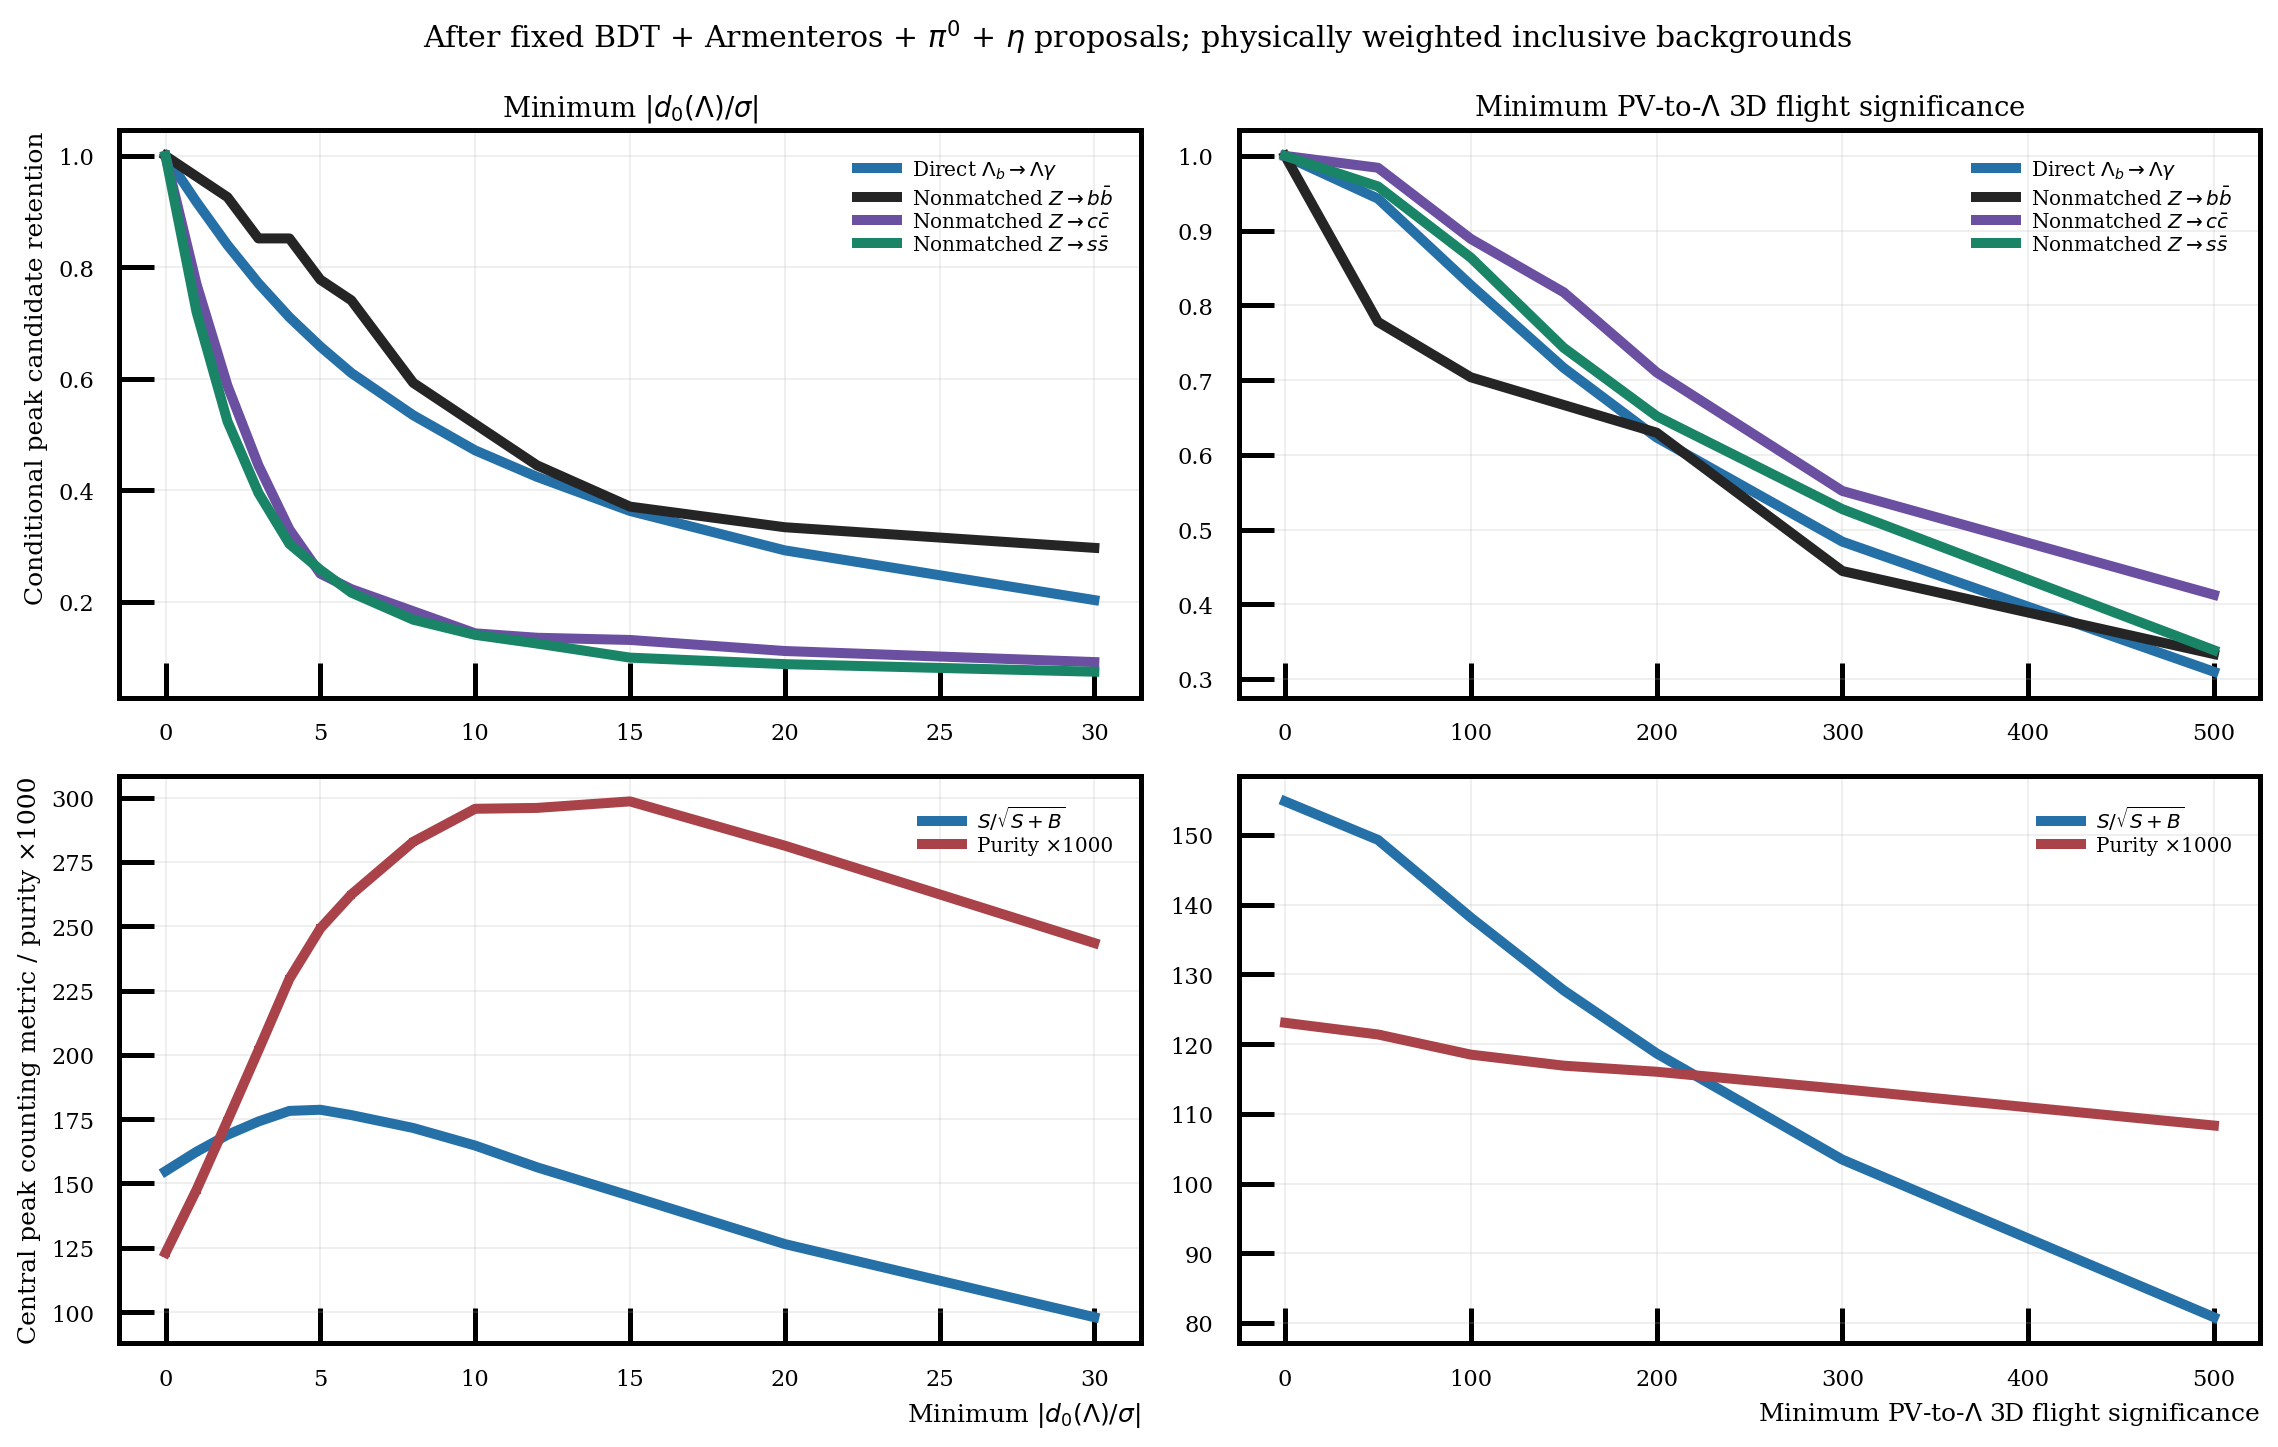
\includegraphics[height=.70\textheight]{figures/displacement_retention_linear.png}
\vspace{.2em}

\scriptsize Paired scan after BDT + Armenteros + $\pi^0$ + $\eta$ proposals. $|d_0(\Lambda)/\sigma|\geq5$ retains 65.8\% signal and 25.7\% Zss peak rows; PV-to-SV flight significance adds little.
\end{frame}

\begin{frame}{Paired mass and angle: illustrative $|d_0/\sigma|\geq5$}
\centering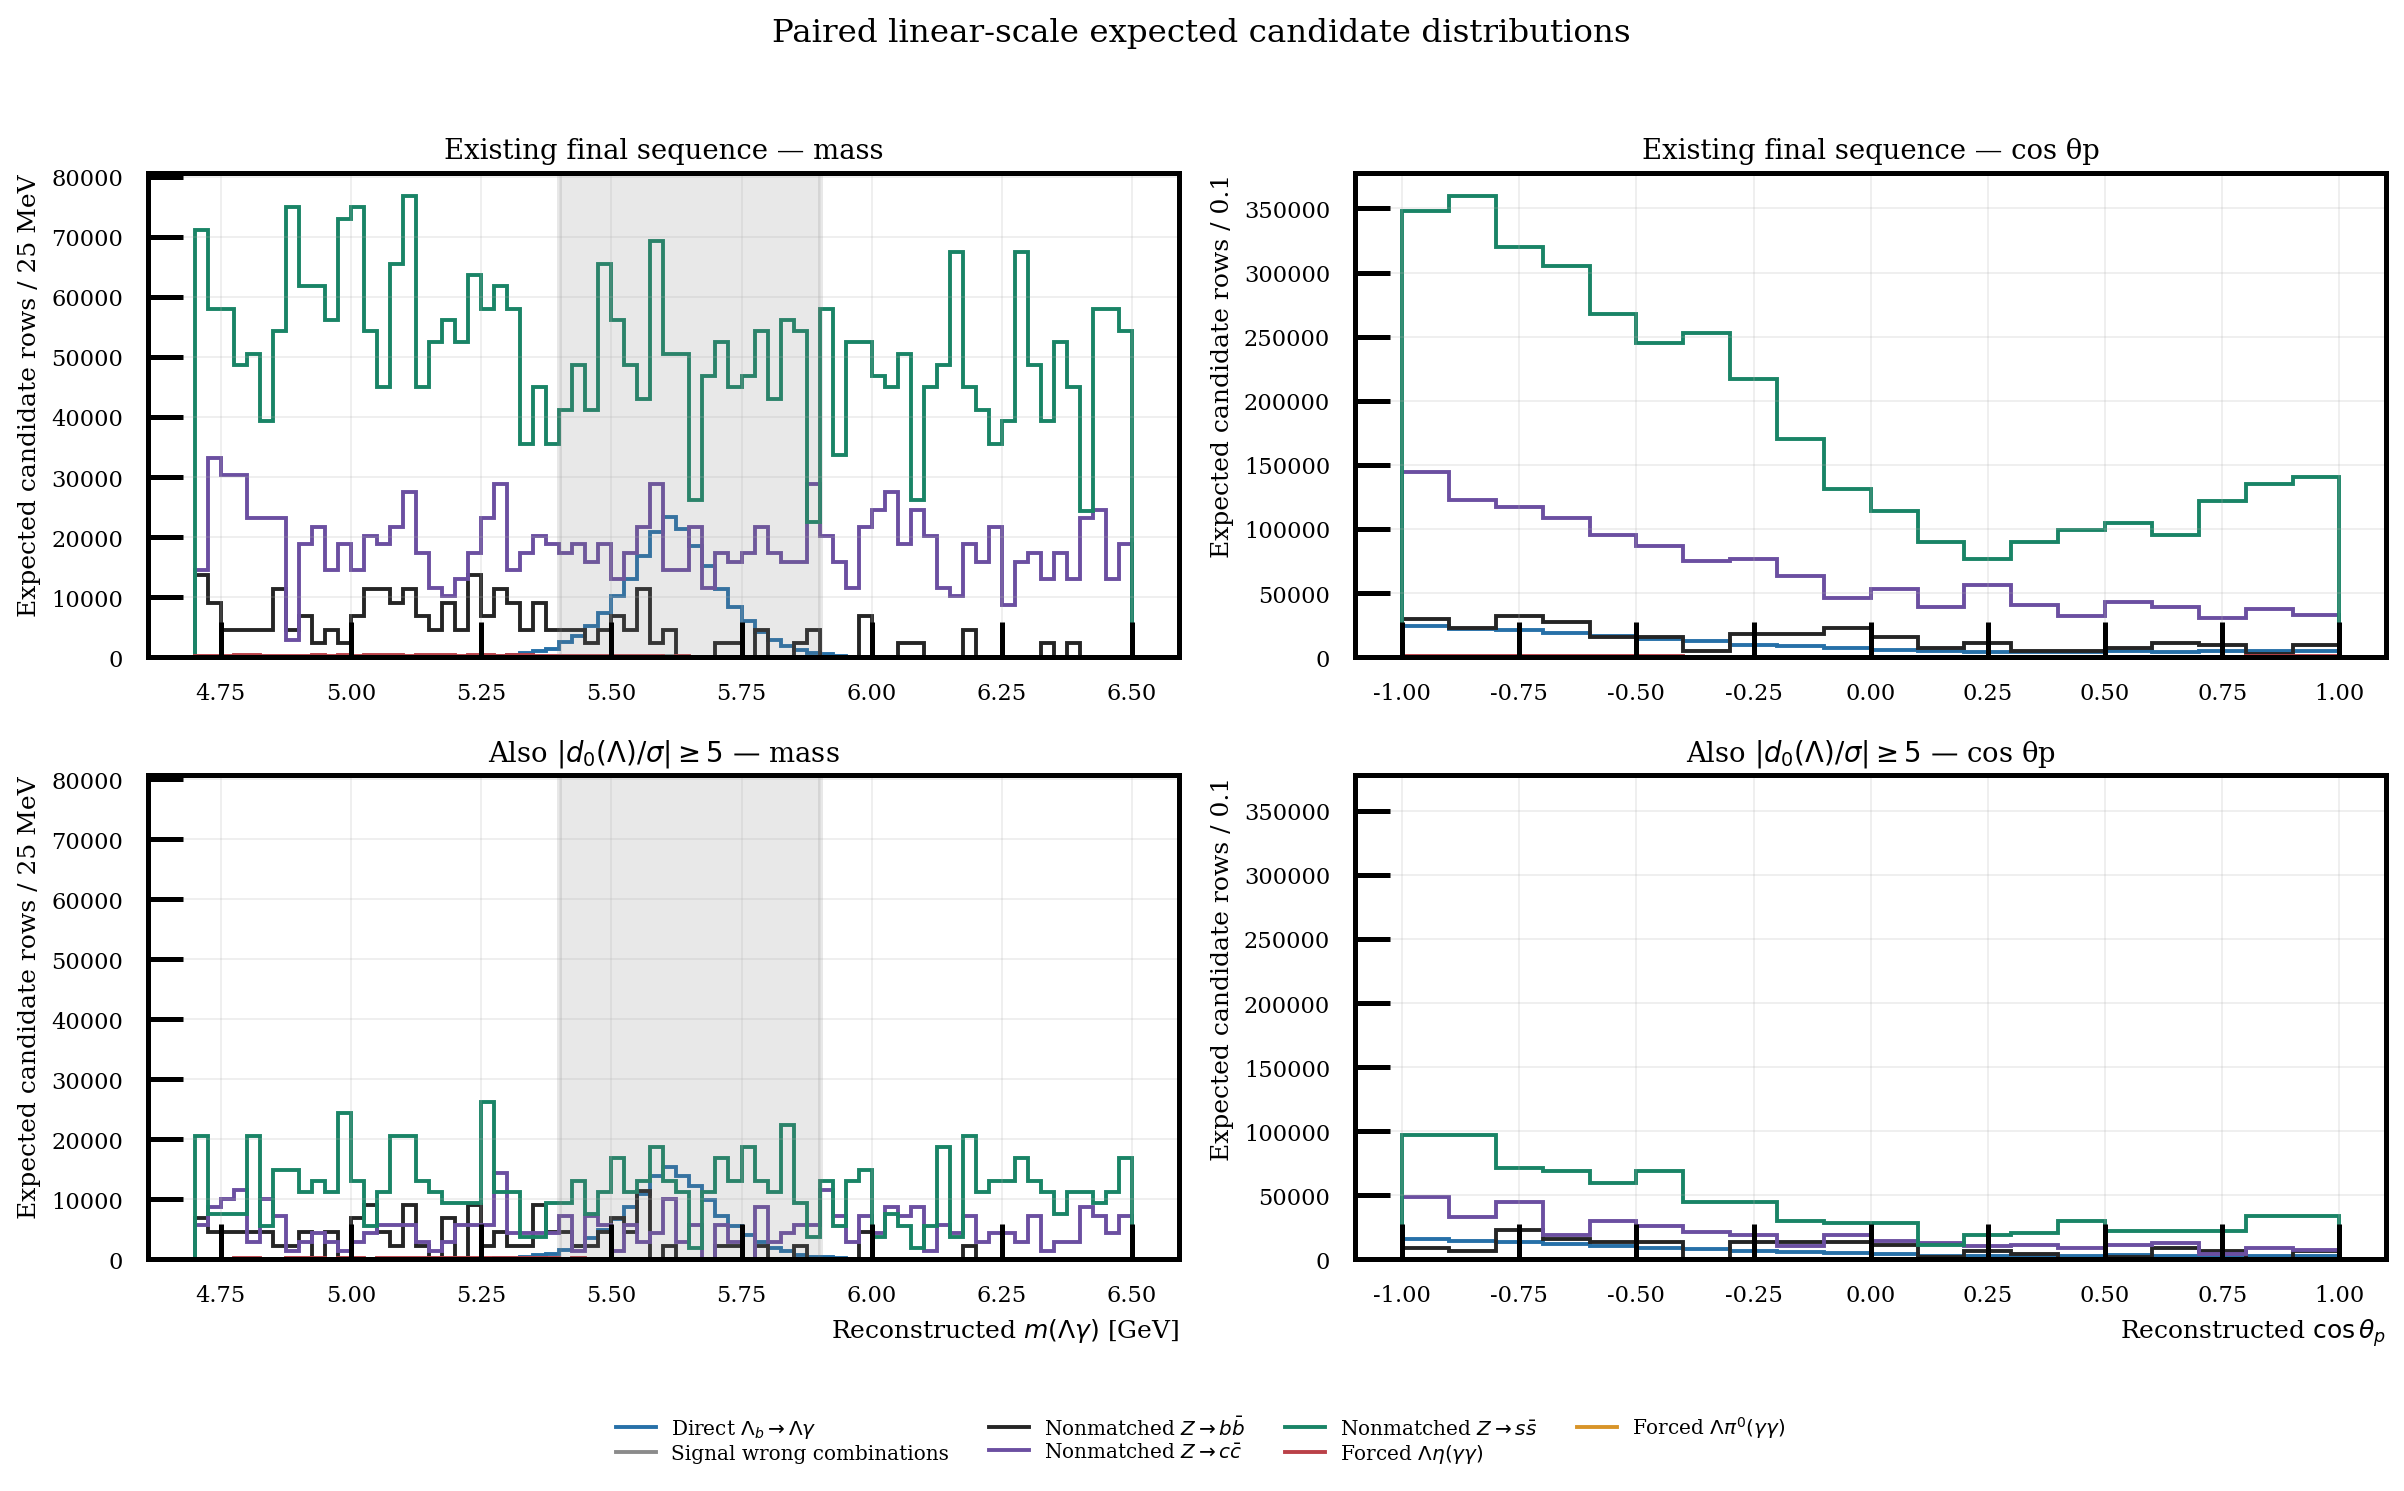
\includegraphics[height=.82\textheight]{figures/mass_angle_d0sig5_linear.png}
\end{frame}

\begin{frame}{Interpretation and PI decision}
\begin{itemize}
\item Zss is the largest projected peak component under the stated branching scenario. An eventual weighted BDT mixture should follow dedicated Zss ancestry and independent test studies.
\item The $\pi^0$ veto retains 98.9\% of direct signal after Armenteros and 88.0\% of Zss. The subsequent $\eta$ veto retains 85.1\% of signal and 73.5\% of Zss while rejecting 80.3\% of forced $\eta$.
\item $S/(S+B_{bb}+B_{cc}+B_{ss})$ rises from 7.9\% at fixed BDT to 12.3\% after all proposals. This excludes forced modes to avoid double counting and is not a fit purity.
\item Decide whether to optimize veto windows and repeat PHSP angular acceptance and resolution checks. No score or veto is adopted by this deck.
\item The additional $\Lambda$ impact-parameter threshold is exploratory. Validate independently, check PV/SV resolution and recompute PHSP angular acceptance before adopting it.
\end{itemize}
\end{frame}
\end{document}
